\section{\texorpdfstring{$\hdhkunit$}{HDH-unit-pack}}
\label{sec:hdhkunit}

This section gives a precise description of $\hdhkunit$ (see \cref{sec:hdhk-prelims:hdhkunit})
and proves its correctness.

\subsection{Shelf-Based Packing}
\label{sec:shelf}

A packing of 2D items in a bin (or strip) is said to be \emph{shelf-based} iff
the bin can be decomposed into regions, called shelves, using horizontal cuts,
and the bottom edge of each item touches the bottom edge of some shelf.
See \cref{fig:shelf-based} for an example.
Next-Fit Decreasing Height (NFDH) and First-Fit Decreasing Height (FFDH)%
~\cite{coffman1980performance} are well-known shelf-based algorithms for 2BP and 2SP.

\begin{figure}[!ht]
\centering
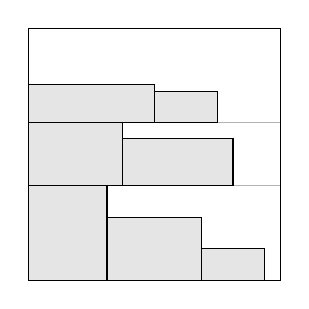
\begin{tikzpicture}[scale=0.8,
shelf-line/.style = {draw={black!30}},
item/.style = {fill={black!10}}
]
\draw[shelf-line] (0,1.5) -- (4,1.5);
\draw[shelf-line] (0,2.5) -- (4,2.5);
\draw (0,0) rectangle (4,4);
\draw[item]
    (0,0) rectangle +(1.25,1.5)
    (1.25,0) rectangle +(1.5,1)
    (2.75,0) rectangle +(1,0.5);
\draw[item]
    (0,1.5) rectangle +(1.5,1)
    (1.5,1.5) rectangle +(1.75,0.75);
\draw[item]
    (0,2.5) rectangle +(2,0.6)
    (2,2.5) rectangle +(1,0.5);
\end{tikzpicture}

\caption{An example of shelf-based packing for $d=2$ with 3 shelves.}
\label{fig:shelf-based}
\end{figure}

The definition of shelf-based packing can be extended to $d$D for $d \ge 1$.
For $d=1$, every packing is said to be a shelf-based packing.
For $d \ge 2$, for a $d$D cuboid, there are two faces of the cuboid that are
perpendicular to the $d\Th$ dimension. The face with the smaller $d\Th$ coordinate
is called the \emph{base} of the cuboid.
A packing of $d$D items into a bin is shelf-based iff the $d$D bin
can be split into $d$D shelves using hyperplanes perpendicular to the $d\Th$ dimension,
and the base of each item is placed on the base of some shelf.

A packing of $d$D items into a bin is \emph{recursive-shelf-based} iff
the packing is shelf-based and the packing of the bases of items on the base of each shelf
is a $(d-1)$D recursive-shelf-based bin packing.
(For $d=1$, every packing is said to be recursive-shelf-based.)

This helps us reduce $d$BP to $(d-1)$BP, $(d-1)$BP to $(d-2)$BP, and so on.
The algorithm $\hdhk$ by Caprara~\cite{caprara2008}
outputs a recursive-shelf-based packing by using this strategy.

\subsection{Description and Analysis of \texorpdfstring{$\hdhkunit$}{HDH-unit-pack}}

For a $d$D item $i$, define $i^{(j)}$ as the $j$D item
obtained by ignoring all dimensions of $i$ other than the first $j$.
For a set $I$ of $d$D items, let $I^{(j)} \defeq \{i^{(j)}: i \in I\}$.

$\hdhkunit$ takes as input a set $I$ of $d$D items,
where all items in $I$ have the same type vector and $\vol(f_k(I - \{\last(I)\})) < 1$.
$\hdhkunit(I)$ works recursively on $d$.
When $d = 1$, it simply returns $I$.
When $d > 1$, it first sorts $I$ in decreasing order of $d\Th$ dimension
if $\type_k(\ell_d(i)) = k$ for each item $i \in I$.
It then repeatedly picks the smallest prefix $J$ of $I$ such that $\vol(f_k(J^{(d-1)})) \ge 1$,
and packs $J$ into a $d$D shelf.
It packs all those shelves into a $d$D bin and returns that packing.
See \cref{algo:hdhkunit} for a more precise description.

\begin{algorithm}[!ht]
\caption{$\hdhkunit^{[t]}(I)$:
For any $d \ge 1$, returns a recursive-shelf-based packing of $I$ into a $d$D bin,
where $I$ is a sequence of $d$D cuboidal items
and $\vol(f_k(I-\{\last(I)\})) < 1$.
Here $\last(I)$ is the last item in sequence $I$.
Also, all items in $I$ have the same type $t$, i.e.,
$\forall i \in I, \type(i) = t$.}
\label{algo:hdhkunit}
\begin{algorithmic}[1]
\If{$d \texttt{ == } 1$}
    \Comment{when items are 1D}
    \State \Return $I$.
    \Comment{\cref{thm:hdhkunit} proves that they fit in a bin.}
\EndIf
\If{$t_d \texttt{ == } k$}
    \Comment{when length in $d\Th$ dimension is small}
    \State \label{alg-line:hdhunit:sort}Sort $I$ in decreasing order of $d\Th$ dimension.
\EndIf
\Comment{otherwise don't disturb ordering of items.}
\State Let $P$ be an empty list.
\While{$|I| > 0$}
    \State \label{alg-line:hdhunit:prefix}Find $J$, the smallest prefix of $I$ such that
        $J = I$ or $\vol(f_k(J^{(d-1)})) \ge 1$.
    \State Let $t'$ be a $(d-1)$-dimensional vector obtained by
        removing the $d\Th$ entry from $t$.
    \State \label{alg-line:hdhunit:recurse}$S = \hdhkunit^{[t']}(J^{(d-1)})$
        \Comment{$S$ is a $d$D shelf containing items $J$.}
    \State Append $S$ to the list $P$.
    \State Remove $J$ from $I$.
\EndWhile
\State Return the shelf packing $P$.
\Comment{\cref{thm:hdhkunit} proves that the sum of heights of shelves doesn't exceed 1,
so this is a valid packing.}
\end{algorithmic}
\end{algorithm}

Define $\wfk(i)$ to be the cuboid $\itild$ where $\ell_j(\itild) \defeq f_k(\ell_j(i))$
for $j \in [d-1]$ and $\ell_d(\itild) \defeq \ell_d(i)$.
Define $\wfk(I) \defeq \{\wfk(i): i \in I\}$.

\begin{theorem}[Correctness]
\label{thm:hdhkunit}
For a set $I$ of $d$D cuboidal items, if $\vol(f_k(I-\{\last(I)\})) < 1$,
then $\hdhkunit(I)$ can pack $I$ in a $d$D bin.
\end{theorem}
\begin{proof}
Let us prove this by induction on $d$.
%See proof of lemma 4.1 in \cite{caprara2008}.
Let $\mathcal{P}(d)$ be this proposition:
For every sequence $I$ of $d$D items, if $\vol(f_k(I)) < 1 + \vol(f_k(\last(I)))$,
then $\hdhkunit(I)$ can pack $I$ into a $d$D bin.

\textbf{Base case}:
Let $I$ be a sequence of 1D items such that $\vol(f_k(I)) < 1 + \vol(f_k(\last(I)))$.

Suppose $t_1 \neq k$.
Then for all $i \in I, \vol(i) \le 1/t_1 = \vol(f_k(i))$. Therefore,
\begin{align*}
& \vol(f_k(I)) < 1 + \vol(f_k(\last(I)))
\\ &\implies \frac{|I|}{t_1} < 1 + \frac{1}{t_1}
\\ &\implies |I| < t_1 + 1 \implies |I| \le t_1
\\ &\implies \vol(I) \le \frac{|I|}{t_1} \le 1.
\end{align*}
Since $\vol(I) \le 1$, $I$ fits in a bin.

Suppose $t_1 = k$.
Then for all $i \in I, \vol(f_k(i)) = \frac{k}{k-2}\vol(i)$. Therefore,
\begin{align*}
\vol(I) &= \frac{k-2}{k}\vol(f_k(I))
\\ &< \frac{k-2}{k}\left( 1 + \vol(f_k(\last(I)))\right)
\\ &= \frac{k-2}{k} + \vol(\last(I))
\\ &\le \frac{k-2}{k} + \frac{1}{k} < 1.
\end{align*}
Since $\vol(I) \le 1$, $I$ fits in a bin.
Therefore, $\mathcal{P}(1)$ holds.

\textbf{Inductive step}:\\
Let $d \ge 2$ and assume $\mathcal{P}(d-1)$ holds.
Let $I$ be a sequence of $d$D items such that $\vol(f_k(I)) < 1 + \vol(f_k(\last(I)))$.
$\mathcal{P}(d-1)$ implies that $\hdhkunit(I)$ doesn't fail at
line \ref{alg-line:hdhunit:recurse}.
Let $s \defeq \last(I)$.

For $i \in I$, define $w(i) \defeq \prod_{j=1}^{d-1} f_k(\ell_j(i))$
and for $X \subseteq I$, define $w(X) \defeq \sum_{i \in X} w(i)$.
Let there be $p$ shelves in the list $P$.
Let $S_j$ be the $j\Th$ shelf that was added to $P$.
Given the way each prefix is chosen in line \ref{alg-line:hdhunit:prefix},
\begin{equation}\label{eqn:hdhunit:shelf-wide}
\forall j \le p-1, w(S_j) \ge 1 \end{equation}
Define $\ell_d(S_j) \defeq \max_{i \in S_j} \ell_d(i)$ to be the height of shelf $S_j$.
Let $H$ be the total height of the shelves, i.e. $H \defeq \sum_{j=1}^p \ell_d(S_j)$.
Then we need to prove that the shelves fit in the bin, i.e. $H \le 1$.

\textbf{Case 1}: Suppose $t_d \neq k$.\\
Then $\forall i \in I, \ell_d(i) \le 1/t_d = f_k(\ell_d(i))$. Therefore,
\[ 1 > \vol(f_k(I-s)) = \frac{w(I-s)}{t_d} \implies w(I-s) < t_d. \]
Since ordering of items is not disturbed, $s \in S_p$. Therefore,
\begin{align*}
& t_d > w(I-s) = \sum_{j=1}^{p-1} w(S_j) + w(S_p - s) \ge p-1
\tag{by (\ref{eqn:hdhunit:shelf-wide})}
\\ &\implies p < t_d + 1 \implies p \le t_d
\\ &\implies H = \sum_{j=1}^p \ell_d(S_j) \le \frac{p}{t_d} \le 1.
\tag{$\forall i \in I, \ell_d(i) \le 1/t_d$}
\end{align*}
Since $H \le 1$, the shelves fit in a $d$D bin.

\textbf{Case 2}: Suppose $t_d = k$.\\
Then $\forall i \in I, f_k(\ell_d(i)) = \frac{k}{k-2}\ell_d(i)$. Therefore,
\begin{align}
\vol(\wfk(I)) &= \sum_{i \in I} w(i)\ell_d(i)
= \frac{k-2}{k} \sum_{i \in I} w(i)f_k(\ell_d(i))
= \frac{k-2}{k} \vol(f_k(I))
\nonumber
\\ \label{eqn:hdhunit:wfk-last}
&< \frac{k-2}{k} (1 + \vol(f_k(s)))
= \frac{k-2}{k} + \vol(\wfk(s)).
\end{align}
Since items in $I$ were sorted in decreasing order of $\ell_d$
(line \ref{alg-line:hdhunit:sort}),
$\forall i \in S_j, \ell_d(i) \ge \ell_d(S_{j+1})$.
Then by (\ref{eqn:hdhunit:shelf-wide}), we get that for all $j \in [p-1]$,
\begin{equation}
\label{eqn:hdhunit:wfk-lb-height}
\vol(\wfk(S_j)) \ge w(S_j)\ell_d(S_{j+1}) \ge \ell_d(S_{j+1})
\end{equation}
Therefore,
\begin{align*}
H &= \sum_{j=1}^{p} \ell_d(S_j)
\le \frac{1}{k} + \sum_{j=1}^{p-1} \ell_d(S_{j+1})
\tag{since $\ell_d(S_1) \le 1/k$}
\\ &\le \frac{1}{k} + \sum_{j=1}^{p-1} \vol(\wfk(S_j))
\tag{by (\ref{eqn:hdhunit:wfk-lb-height})}
\\ &< \frac{1}{k} + \vol(\wfk(I))
\\ &< \frac{1}{k} + \frac{k-2}{k} + w(s)\ell_d(s)
\tag{by (\ref{eqn:hdhunit:wfk-last})}
\\ &\le \frac{k-1}{k} + \frac{1}{k} = 1.
\tag{since $\ell_d(s) \le 1/k$ and $w(s) = \vol(f_k(s^{(d-1)})) \le 1$}
\end{align*}
Since $H \le 1$, the shelves fit in a $d$D bin.
Therefore, $\mathcal{P}(d)$ holds.

Therefore, by mathematical induction, $\mathcal{P}(d)$ holds for all $d \ge 1$.
\begin{optional}
We can generalize the definition of $f_k$ by replacing $k/(k-2)$ by $\mu$, where $\mu \le k$.
The base case and case 1 of the inductive step require $\mu \ge k/(k-1)$.
Case 2 of the inductive step requires $\mu \ge k/(k-2)$;
we will show how to weaken this requirement.

Case 2 implies that $\forall i \in I, f_k(\ell_d(i)) = \mu\ell_d(i)$. Therefore,
\begin{align}
\vol(\wfk(I)) &= \sum_{i \in I} w(i)\ell_d(i)
= \frac{1}{\mu} \sum_{i \in I} w(i)f_k(\ell_d(i))
= \frac{1}{\mu} \vol(f_k(I))
\nonumber
\\ \label{eqn:hdhunit:wfk-last-2}
&< \frac{1}{\mu} (1 + \vol(f_k(s)))
= \frac{1}{\mu} + \vol(\wfk(s)).
\end{align}

\textbf{Case 2a}: $\forall j \in [d-1], t_j \neq k$.\\
Let $T \defeq \prod_{j=1}^{d-1} t_j$.

Since items in $I$ were sorted in decreasing order of $\ell_d$
(line \ref{alg-line:hdhunit:sort}),
$\forall i \in S_j, \ell_d(i) \ge \ell_d(S_{j+1})$.
Since $t_j < k$ for $j \in [d-1]$, $w(i) = 1/T$ for each item $i \in I$.
Given the way each prefix is chosen in line \ref{alg-line:hdhunit:prefix},
$|S_j| = T$ for $j \in [p-1]$. Therefore, for all $j \in [p-1]$,
there is one item of height $\ell_d(S_j)$ in $S_j$
and all the other $T-1$ items in $S_j$ have height at least $\ell_d(S_{j+1})$.
This gives us
\[ \vol(\wfk(S_j)) = \sum_{i \in S_j} \frac{\ell_d(i)}{T}
\ge \frac{1}{T}\ell_d(S_j) + \frac{T-1}{T}\ell_d(S_{j+1}). \]
\begin{align*}
\vol(\wfk(I)) &= \sum_{j=1}^{p-1} \vol(\wfk(S_j)) + \vol(\wfk(S_p))
\\ &\ge \sum_{j=1}^{p-1} \left(\frac{1}{T}\ell_d(S_j) + \frac{T-1}{T}\ell_d(S_{j+1})\right)
    + \frac{1}{T}\ell_d(S_p)
\\ &= \frac{1}{T}\sum_{j=1}^p \ell_d(S_j) + \frac{T-1}{T}\sum_{j=1}^{p-1}\ell_d(S_{j+1})
\\ &= H - \frac{T-1}{T}h(S_1)
\ge H - \frac{T-1}{T}\frac{1}{k}.
\end{align*}
\begin{align*}
H &\le \vol(\wfk(I)) + \frac{T-1}{T}\frac{1}{k}
\\ &< \frac{1}{\mu} + \vol(\wfk(s)) + \frac{T-1}{T}\frac{1}{k}
\tag{by (\ref{eqn:hdhunit:wfk-last-2})}
\\ &\le \frac{1}{\mu} + \frac{1}{T}\frac{1}{k} + \frac{T-1}{T}\frac{1}{k}
\tag{since $w(s) = 1/T$ and $\ell_d(s) \le 1/k$}
\\ &= \frac{1}{\mu} + \frac{1}{k}.
\end{align*}
Since we want $H \le 1$, we get $\mu \le k/(k-1)$.

\textbf{Case 2b}: $\exists q \in [d-1], t_q = k$.
\begin{align*}
H &= \sum_{j=1}^p \ell_d(S_j)
\le \frac{1}{k} + \sum_{j=1}^{p-1} \ell_d(S_{j+1})
\tag{since $\ell_d(S_1) \le 1/k$}
\\ &\le \frac{1}{k} + \sum_{j=1}^{p-1} \vol(\wfk(S_j))
\tag{by (\ref{eqn:hdhunit:wfk-lb-height})}
\\ &< \frac{1}{k} + \vol(\wfk(I))
\\ &< \frac{1}{k} + \frac{1}{\mu} + w(s)\ell_d(s)
\tag{by (\ref{eqn:hdhunit:wfk-last-2})}
\\ &\le \frac{1}{k} + \frac{1}{\mu} + \frac{\mu}{k^2}.
\tag{since $\ell_d(s) \le 1/k$ and $w(s) \le f_k(\ell_q(s)) \le \mu/k$}
\end{align*}
For $H \le 1$ and $\mu \le k$, we get $k \ge 3$ and
\[ \mu \ge \frac{k((k-1) - \sqrt{(k-3)(k+1)})}{2}
    \le \frac{k(k-2)}{k^2-3k+1} \le \frac{k}{k-2}. \]
\end{optional}
\end{proof}

Note that $\hdhkunit$ has a running time of $O(n\log n)$.

\textbf{Comment on Caprara's~\cite{caprara2008} analysis of $\hdhk$.}
Caprara~\cite{caprara2008} implicitly proves \cref{thm:hdhkunit} in Lemma 4.1 in their paper
and their proof is less detailed than ours.
Their algorithm is similar to ours, except that
they allow arbitrarily reordering $I$ when $t_d \neq k$,
and instead of choosing a prefix of $I$
(line \ref{alg-line:hdhunit:prefix} in $\hdhkunit$),
they choose a subset of $I$ that is minimal for some properties.
